\chapter{State of the art} \label{state_of_the_art}

In this chapter is of the utmost importance to define some concepts that were used as a basis for this thesis. 
In addition, it will be discussed possible tools that already answer some of the questions that this thesis is trying to answer, and for that matter are important to be studied and referenced.
	

\section{Context-free Grammar}

A Grammar can be defined by the study and learning of the way sentences of a language are assembled.
The word ``grammar'' is extracted from the Greek \emph{Tékhnē grammatikē}), which has the meaning of ``art of letters'' \cite{britannica_2020}.
This can be interpreted has the art of combining letters in order to produce a system which determines the correct way of constructing phrases.
A grammar does not assign any meaning for these phrases (semantic), it only structures their form.

A Context-free Grammar (\textsc{CFG}) is defined by a tuple of 4 elements \cite{henriques_2011}

\[ G = (T, N, S, P) \]

\noindent where \textbf{T} is the set of terminal symbols of a language;
\textbf{N} is the set of non-terminal symbols;
\textbf{S} is the start symbol of the grammar;
\textbf{P} is the set of productions that compose this grammar.
The productions within the grammar are rules of form

\[ N \rightarrow (N \cup T)^* \]

\noindent where the left side, composed of a non-terminal symbol, may derive in a set of non-terminal and terminal symbols.


\section{Attribute Grammars}
Attribute Grammars were proposed by Donald Knuth in order to specify static and dynamic semantics of a programming language in a syntax-directed manner \cite{thirunarayan_2009}. 
The process consists in constructing the syntax tree and then computing the values of attributes by visiting every single node. 
For each attribute it is possible to associate a domain of values, such as integers, strings or even complex structures. 

\noindent Formally an attribute grammar (AG) is a tuple \cite{pereira_2016}

\[ AG = (CFG, A, CR, CC, TR) \]

\noindent composed by a context-free grammar (CFG), which has been extended to provide context by using a set of attributes; 
The set of attributes (A), which exist in each production of a grammar, are divided into two groups, \emph{Synthezized Attributes}, which allow values to be passed from one node to its parent, 
and \emph{Inherited Attributes}, which allow values to be passed from the current node to a child \cite{slonneger_1995}; 
rules for calculating attributes (CR) in all productions of the grammar; 
a set of contextual conditions (CC); 
and the transformation rules (TR) in all productions of the grammar.


\section{Domain Specific Languages}
A domain specific language is an ``executable specification language, through appropriate notations and abstractions'', usually restricted to a particular problem domain. 
Its objective is to improve productivity, and to allow solutions to be expressed in a more intuitive way and at the level of abstraction of the problem domain \cite{van_2000}.
These types of languages provide a natural vocabulary for concepts that are fundamental to the problem scope \cite{bruce_1997}, something that may lack when using a general-purpose language. 
\textsc{DSLs} are usually small and declarative, with very specific goals \cite{van_2000}.
Refered as ``little languages'' \cite{bentley_1986}, they are intended to solve problems within a specific domain, and not outside it.

One of the disadvantages of building a new \textsc{DSL} is the cost of their development, as it requires both domain and language development expertise \cite{kosar_2008},
so the commitment of using \textsc{DSL}s as a solution for a software problem if often postponed or not even comtemplated.
Nevertheless, as \textsc{DSL}s trade generality, they gain expressiveness (in a limited domain) - this results in the ease of repetitive tasks and smoother data
description \cite{mernik_2005} and representation.

As discussed in \cite{barisic_2012}, usability should be embedded in the \textsc{DSL} development process itself, and considered from the beginning of its development.
The new created \textsc{DSL} needs to identify the problems within the domain, trying to overcome them while maintaining the expected expressivity.


\section{PAG (Prototyping with Attribute Grammars)}
PAG is a tool that was created with the purpose of helping two distinct groups of students from \emph{Universidad Complutense de Madrid}. 
One of those groups, involving computer science students, that attended a class which teached compiler contructions, and other group involving linguistic students, from a class on computacional linguistics. 
Teachers from both classes used the same methodology to teach their classes, 
and noticed that it wasn't good enough for the students to master all the concepts: On one hand, they would have computer science skilled students, 
with great apititude to produce solutions, but leaving aside the respective specifications, which lead to poor and innacurate formal specifications, but on the other hand, 
linguistic students produced good formal specifications, as they are proficient with the natural language,
but lack computer science skills to well transpose all the knowledge into computacional models \cite{sierra_2006}.
	
The result was an environment based in attribute grammars that allows the specification of those same grammars using a language close to Prolog. 
The main goal was to embed Prolog into the language and maintain all the familiar basic notation, 
the reason being both groups of students were already familiar with the Prolog and attribute grammar syntax and notation. 
Through rapid prototyping, which PAG makes use of, it is possible to obtain a functional processor at a embryonic state of the problem \cite{sierra_2006}. 
With this, computer science students can obtain results quite early, allowing them to apply more time into formal specifications. 
Moreoever, as the complexity of the syntax is reduced, this allows for a better and easier learning experience for students which have less aptitude for the solution codification or programming in general, 
which is the case for linguistic students.

Overall, PAG solved the problem that was purposed in an effective way. 
Despite that, and giving the respective credit to the those who built the tool, the fact is that Prolog can still be quite difficult to grasp for some people, and a challenge when it comes to learn it. 
The usage of a specification language that closely resembles the natural one, could be a great addition.


\section{CONSTRUCTOR}
CONSTRUCTOR \cite{alexin_1990} is a Natural Langugage Interface that accepts and processes English sentences,
using them as instructions for plane geometry constructing.
Those instructions are then transformed into the respective graphical representation.
The idea is that these sentences are issued as commands which represent steps for the creation of a geometrical construction.
CONSTRUCTOR analyses the issued inpu, translates it into a semantic representation and, based on that semantic representation, builds a visual construction.
Furthermore, CONSTRUCTOR keeps track of the sequence of inputs issued by the user, which results in a more controlled construction process,
while giving the user feedback within each step.

\noindent CONSTRUCTOR is composed by the following parts:

\begin{itemize}
	\item \textbf{Lexical Analyser} - consists in a machine dictionary of more than 300 items that are usually necessary for issuing commands.
		It also stores synonyms of the various items, as different people (based on age or level of training) may use different (but similar) words.
		This module is also extended by a morphological analyser, which analyses words that are not present in the dictionary,
		extracting its canonical lexeme an then perform an evaluation.
	
	\newpage
	\item \textbf{Syntactic Parser} - a string of tokens and terminals is used as input for the syntactic parser.
		This string is then processed into a sentence (or list of) with some structure assigned to it.
		All sentences must only describe one step and one step only, but nested sentences are possible.
		Below there is a table, extracted for the article (\cite{alexin_1990}) that shows various sentences examples.
		\begin{figure}[h]
			\centering
			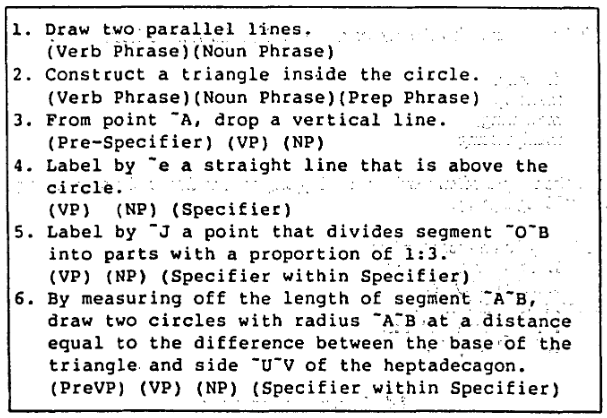
\includegraphics[width=10cm]{images/constructor_sentence_struct.png}
			\caption{Example of structured input sentences for CONSTRUCTOR.}
			\label{fig:constructorSentenceStruct}
		\end{figure}

	\item \textbf{Attribute Evaluation} - computes the basic features of grammatical structures, such as synthesized attributes.
		This computation will mostly involve synthesized attribute evaluation.

	\newpage
	\item \textbf{Semmantic Interpretation} - the semantic interpreter takes the results of all evaluations done before as input.
		The goal is to transform the English sentences into a \textit{metalevel} description intended for building complex noun phrases.
		\begin{figure}[h]
			\centering
			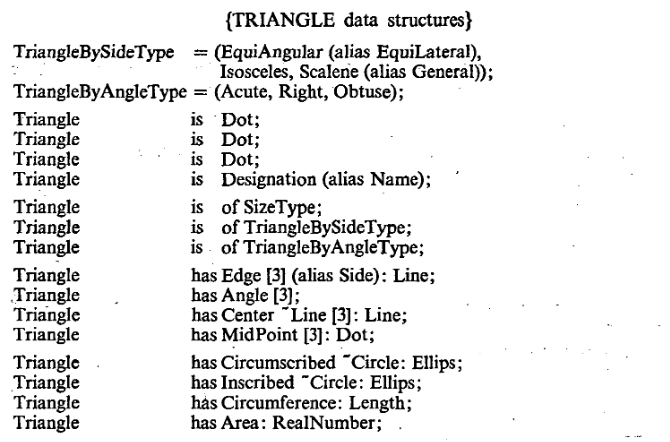
\includegraphics[width=12cm]{images/constructor_metalevel_desc.png}
			\caption{Example of a \textit{metalevel} description of CONSTRUCTOR.}
			\label{fig:constructorMetalevelDesc}
		\end{figure}
	
	\item \textbf{Construction Creator} - final component which takes a formal specification of an object, defining all the procedures to be executed.
		The results is a drawn geometric figure.
\end{itemize}

The purpose of exploring a tool of this type is not directly related to linguistics nor linguistic rules training.
The relevance of this reference is related to the use of attribute grammars with natural language processing, which techniques could be helpful when tacking a specific problem of this kind.


\section{VisualLISA (A Visual Programming Environment for Attribute Grammars)}
VisualLISA is a visual programming environment created by Nuno Oliveira in the year of 2009 \cite{oliveira_2009} for the specification of attribute grammars. 
Classified as a ``Domain Specific  Visual Language'', its main goal was to enhance the front-end of one other tool named LISA \footnote{https://labraj.feri.um.si/lisa/}, 
a compiler generator based in AG's that creates different visual tools based on the textual specification of the grammars.
    
The aim of this tool was to decrease the difficulty which is involved with specifying attribute grammars, not only for the LISA environment, but also regarding other types of systems, 
making specifications more visual and graphical.
    
Specifying grammars in a visual manner can be done using a set of icons (\autoref{fig:visuallisa_icons}) that must be combined to obtain the wanted result. 
Each icon or symbol has a unique function, and it is the users task to make the connections in a correct way.
    
% Imagem dos icons do VisualLISA
\begin{figure}[h]
    \centering
    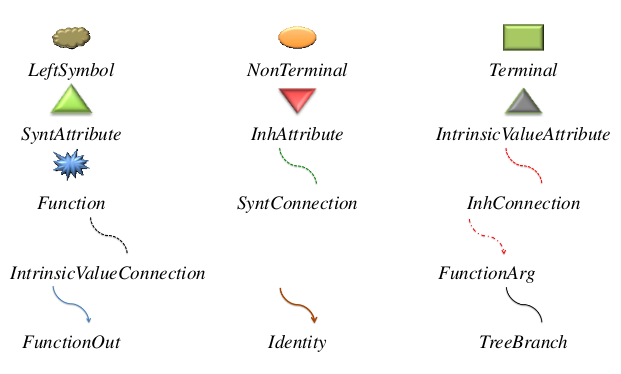
\includegraphics[width=10cm]{images/visuallisa_icons.png}
    \caption{VisualLISA set of icons.}
    \label{fig:visuallisa_icons}
\end{figure}

\newpage
The environment (\autoref{fig:visuallisa_window}) consists in 4 windows, each one with an individual task: 
declare the productions of the grammar in a textual manner; 
declare functions, data-types, etc.; 
draw the grammar productions; 
specify computation rules that were previously declared.
    
% Imagem da janela do VisualLISA
\begin{figure}[h]
    \centering
    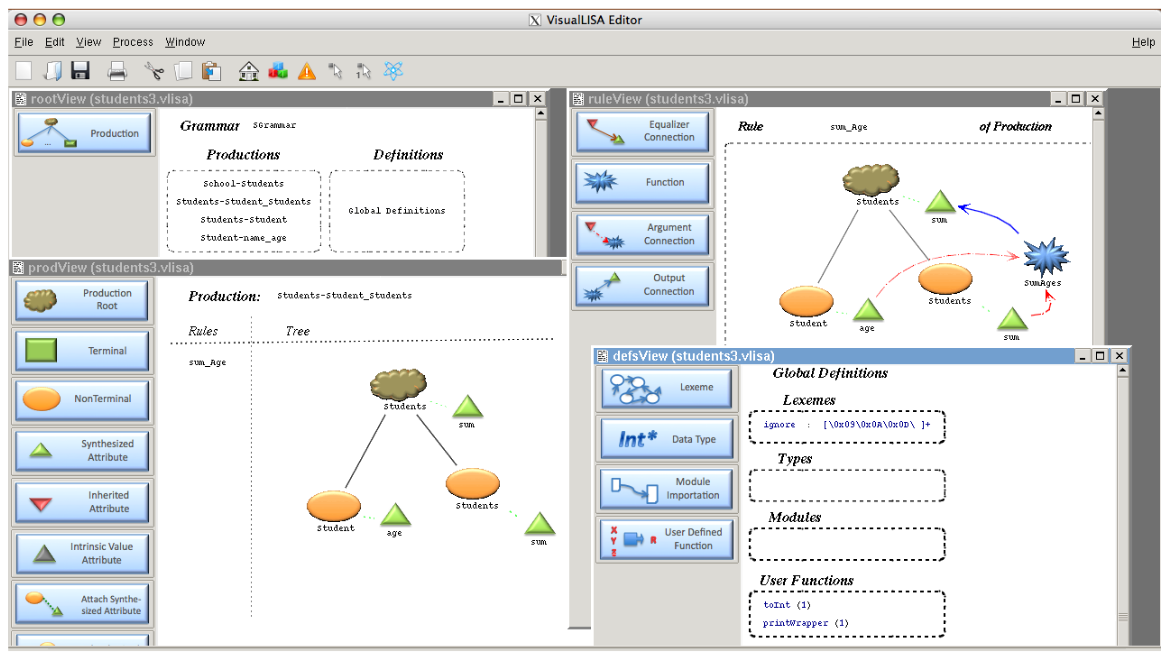
\includegraphics[width=10cm]{images/visuallisa_window.png}
    \caption{VisualLISA main window.}
    \label{fig:visuallisa_window}
\end{figure}
    
As an example, it was included a textual specification (\autoref{fig:textual_students_grammar}) 
and the respective graphical specification (\autoref{fig:graphical_students_grammar}), extracted from the paper \cite{oliveira_2009}.
    
% Students Grammar
\begin{figure}[h]
    \centering
    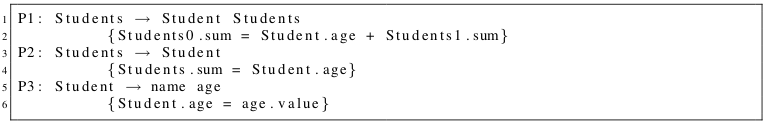
\includegraphics[width=15cm]{images/textual_students_grammar.png}
    \caption{Students textual grammar.}
    \label{fig:textual_students_grammar}
\end{figure}

\newpage

% VisualLISA Conception
\begin{figure}[h]
    \centering
    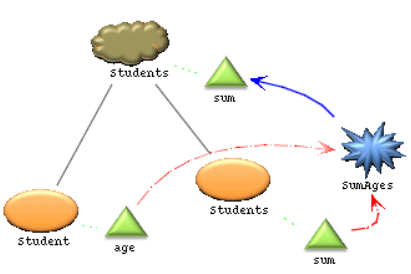
\includegraphics[width=8cm]{images/graphical_students_grammar.png}
    \caption{Students graphical grammar.}
    \label{fig:graphical_students_grammar}
\end{figure}

The main effect of the tool is not directly related to the problem that is trying to be solved, as the target users (linguists) may not be familiar with attribute grammars concepts such as 
terminal or non-terminal.
This can cause some confusion when working with all the icons provided by the platform in order to create the intended atttribute grammar.
Nevertheless, all the visual components that are associated could give some insights of interesting visual components to include/build when creating the proposed user interface to interact with the system.


\section{Chapter Summary} % TALVEZ ACRESCENTAR PEQUENA DESCRIÇÃO DE CADA SISTEMA????

In the previous sections, some tools were presented and major concepts discussed.
Some of the tools may not have a direct impact on the proposal of this thesis, but their research and inclusion on this document were crucial.
Each of the sections, despite their various differences, share the use of attribute grammars as a basis for a particular system,
or even to simplify their use thorugh various techniques.

The solution proposed is an approach that, despite using attribute grammars, 
it is based on a new textual \textsc{DSL} using \textsc{ANTLR} and the automated generation of processors in order to validate sentences.
In the next chapter, the proposal for this particular system will be discussed further.


% what is useful are all the visual components that are associated with it, 
% which could help when creating the intended user interface for the visual analysis of the generated 
% syntax-tree, or more. 
% Nevertheless, it is a very useful and interesting way of aproaching attribute grammars and their 
% specifications.
